%%%%%%%%%%%%%%%%%%%%%%%%%%%%%%%%%%%%%%%%%
% Short Sectioned Assignment
% LaTeX Template
% Version 1.0 (5/5/12)
%
% This template has been downloaded from:
% http://www.LaTeXTemplates.com
%
% Original author:
% Frits Wenneker (http://www.howtotex.com)
%
% License:
% CC BY-NC-SA 3.0 (http://creativecommons.org/licenses/by-nc-sa/3.0/)
%
%%%%%%%%%%%%%%%%%%%%%%%%%%%%%%%%%%%%%%%%%

%----------------------------------------------------------------------------------------
%	PACKAGES AND OTHER DOCUMENT CONFIGURATIONS
%----------------------------------------------------------------------------------------

\documentclass[paper=a4, fontsize=11pt]{scrartcl} % A4 paper and 11pt font size

\usepackage[T1]{fontenc} % Use 8-bit encoding that has 256 glyphs
\usepackage{fourier} % Use the Adobe Utopia font for the document - comment this line to return to the LaTeX default
\usepackage[english]{babel} % English language/hyphenation
\usepackage{amsmath,amsfonts,amsthm} % Math packages

\usepackage{lipsum} % Used for inserting dummy 'Lorem ipsum' text into the template

\usepackage{sectsty} % Allows customizing section commands
\allsectionsfont{\centering \normalfont\scshape} % Make all sections centered, the default font and small caps

\usepackage{graphicx}
\usepackage{fancyhdr} % Custom headers and footers
\pagestyle{fancyplain} % Makes all pages in the document conform to the custom headers and footers
\fancyhead{} % No page header - if you want one, create it in the same way as the footers below
\fancyfoot[L]{} % Empty left footer
\fancyfoot[C]{} % Empty center footer
\fancyfoot[R]{\thepage} % Page numbering for right footer
\renewcommand{\headrulewidth}{0pt} % Remove header underlines
\renewcommand{\footrulewidth}{0pt} % Remove footer underlines
\setlength{\headheight}{13.6pt} % Customize the height of the header

\numberwithin{equation}{section} % Number equations within sections (i.e. 1.1, 1.2, 2.1, 2.2 instead of 1, 2, 3, 4)
\numberwithin{figure}{section} % Number figures within sections (i.e. 1.1, 1.2, 2.1, 2.2 instead of 1, 2, 3, 4)
\numberwithin{table}{section} % Number tables within sections (i.e. 1.1, 1.2, 2.1, 2.2 instead of 1, 2, 3, 4)

\setlength\parindent{0pt} % Removes all indentation from paragraphs - comment this line for an assignment with lots of text

%----------------------------------------------------------------------------------------
%	TITLE SECTION
%----------------------------------------------------------------------------------------

\newcommand{\horrule}[1]{\rule{\linewidth}{#1}} % Create horizontal rule command with 1 argument of height

\title {	
\normalfont \normalsize 
\textsc{Georgia Institute of Technology, College of Computing} \\ [25pt] % Your university, school and/or department name(s)
\horrule{0.5pt} \\[0.4cm] % Thin top horizontal rule
\huge CX4640: Homework 1 \\ % The assignment title
\horrule{2pt} \\[0.5cm] % Thick bottom horizontal rule
}

\author{Nathan Korzekwa} % Your name

\date{\normalsize\today} % Today's date or a custom date

\begin{document}

\maketitle % Print the title

%----------------------------------------------------------------------------------------
%	PROBLEM 1
%----------------------------------------------------------------------------------------

\section{Problem 1}
In this problem, we must assume that $y$ remains constant. That is, given a perturbation $\epsilon$, the input changes from 
$(x, y)$ to $(x + \epsilon, y)$. We must assume that one of them remains constant for $cond(f) = 1/\epsilon$ in all cases.
For example, if both $x$ and $y$ are perturbed by the same value $\epsilon$, our measure of the size, $|x| + |y|$ grows, 
while our function, $f(x, y) = x - y$ remains unchanged.

\
To show that $cond(f) = 1/\epsilon$, first recall the definition of a conditional number:
$$
	\frac{||\Delta{y}|| / ||y||}{||\Delta{\vec{x}}||/||\vec{x}||}
$$

In this problem, this is equivalent to:

$$
	\frac{
			\frac{|x - y - [(x + \Delta{x}) - y]|}{|x - y|}
		 }
		 {
		 	\frac{|\Delta{x}|}{|x| + |y|}
		 }
$$

With some reduction, this becomes:

$$
	\frac{
			\frac{|-\Delta{x}|}{|x - y|}
		 }
		 {
		 	\frac{|\Delta{x}|}{|x| + |y|}
		 }	
$$

Then, substituting values from the problem:

$$
	\frac{
			\frac{|\Delta{x}|}{|\epsilon|}
		 }
		 {
		 	\frac{|\Delta{x}|}{1}
		 }	
$$

Which finally becomes:

$$
	\frac{|\Delta{x}|}{|\Delta{x}||\epsilon|} = 1/|\epsilon| = 1/\epsilon 
$$

From this, we can conclude that subtraction is highly sensitive when the difference between $x$ and $y$ is small, and much less so at higher differences.

%----------------------------------------------------------------------------------------
%	PROBLEM 2
%----------------------------------------------------------------------------------------

\section{Problem 2}

In a floating-point system with $p$ precision, altering the bit at $p - 1$ generates adjacent floating point numbers. With the lower-bound $L$ and the upper-bound $U$ on the exponent, and with $\beta$ as the base, it is easy to see that the smallest and greatest adjacent numbers will have exponents of $L$ and $U$ respectively. 

Two adjacent numbers in the set of smallest adjacencies are:
\begin{align}
	x = \beta^L \\
	y = \beta^L(1 + \frac{1}{\beta^{p - 1}}) \\
	  = \beta^L + \frac{\beta^L}{\beta^{p - 1}}
\end{align}

From this, we find the smallest spacing:
\begin{align}
	|x - y| = \beta^{L - p + 1}
\end{align}

Now that we've found the smallest spacing, the largest spacing is very easy to find:

\begin{align}
		x = \beta^U \\
		y = \beta^U(1 + \frac{1}{\beta^{p - 1}}) \\
		  = \beta^U + \frac{\beta^L}{\beta^{p - 1}}
\end{align}

\begin{align}
	|x - y| = \beta^{U - p + 1}
\end{align}

%------------------------------------------------

%----------------------------------------------------------------------------------------
%	PROBLEM 3
%----------------------------------------------------------------------------------------

\section{Problem 3}
(Parts a and b) \\

Below lies a graph of the errors for different values of $log_{10}(error)$ for different values of $log_{10}(h)$. The results are pretty self-explanatory. Interestingly, the rule of thumb, $h = \sqrt{\epsilon_{mach}}$ is near the minimum error for the regular finite difference equation, but for the centered case, the rule of thumb produces rather high error. \\
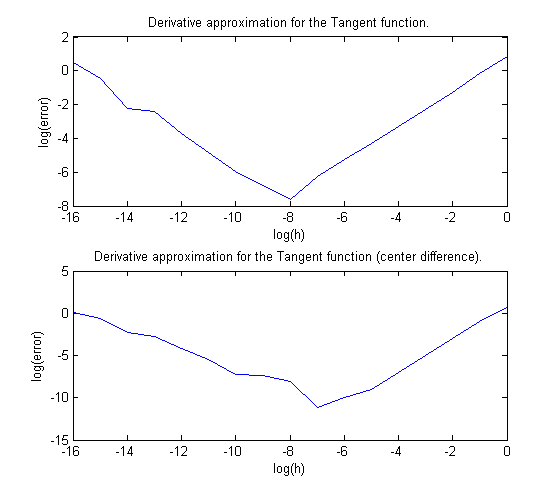
\includegraphics{derivativeGraph} \\
The code that produces this graph can be found in ``q3.m''

%------------------------------------------------

%----------------------------------------------------------------------------------------
%	PROBLEM 4
%----------------------------------------------------------------------------------------

\section{Problem 4}
As can be seen below, the graph does NOT confirm the theoretically expected behavior of the closed-form solution: $x_k = 4^{-k}/3$. \\
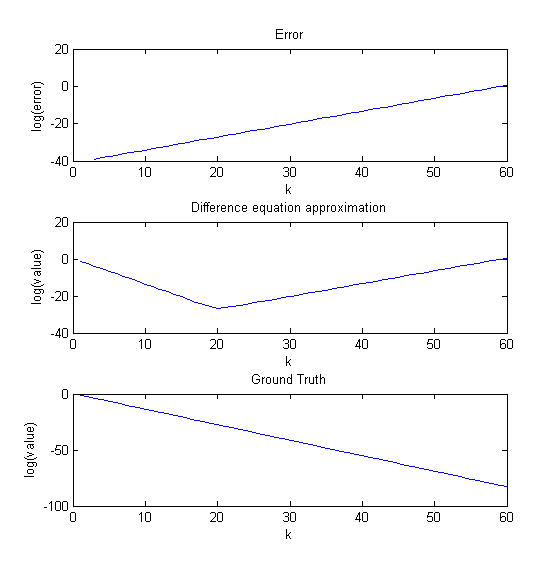
\includegraphics{recurrenceGraph} \\
(The code that produces this graph can be found in ``q4.m'') \\
This is because this particular relation is very sensitive to starting conditions (actually, sooner or later most relations are since they are exponential in nature). However, to geta more clear picture of what's actually happening, let's solve for the general solution of the given recurrence relation. Here, I use Trotter's advancement operator notation.

\begin{align}
	x_{k + 1} = 2.25x_k - 0.5x_{k - 1} \\
	x_{k + 2} = \frac{9}{4}x_{k + 1} - \frac{1}{2}x_{k}
\end{align}
\begin{align}
	x_{k + 2} - \frac{9}{4}x_{k + 1} + \frac{1}{2}x_{k} = 0 \\
	(A^2 - \frac{9}{4}A + \frac{1}{2})x = 0 \\
	\frac{1}{4}[(A - 2)(4A - 1)]x = 0 \\
	A = \frac{1}{4}, 2
\end{align}

So with these roots, the general solution appears to be:
\begin{align}
	x_k = c_1(\frac{1}{4})^k + c_22^k \\
	x_k = c_14^{-k} + c_22^k
\end{align}

With the initial values of $1/3$ and $1/12$, solving for the specific equation annihilates the second term, so the closed-form solution monotonically decreases. However, since floating-point numbers only span a discrete, finite space in $\mathbb{R}$ error begins to accumulate very early in the process, meaning that the effective coefficient $c_2$ is not quite zero. This error is negligible for small $k$, but the exponential growth of $2^k$ quickly grows large enough to become an issue. 


%------------------------------------------------

\end{document}